% Replace 'text' below with your text.  Use \citep{Author2016} to add a
% parenthetical citation; use \citet{Author2016} to get a textual cite like
% this: Author (2016).  FS will add the code to insert figures.

\section{Use Consistent Measures}

\begin{figure}[htbp] 
  \caption{Comparing Three Measures of Rejection of Meritocracy Pooled by \citet{Newman2015}}
  \label{F:three_measures}
  \begin{center}
    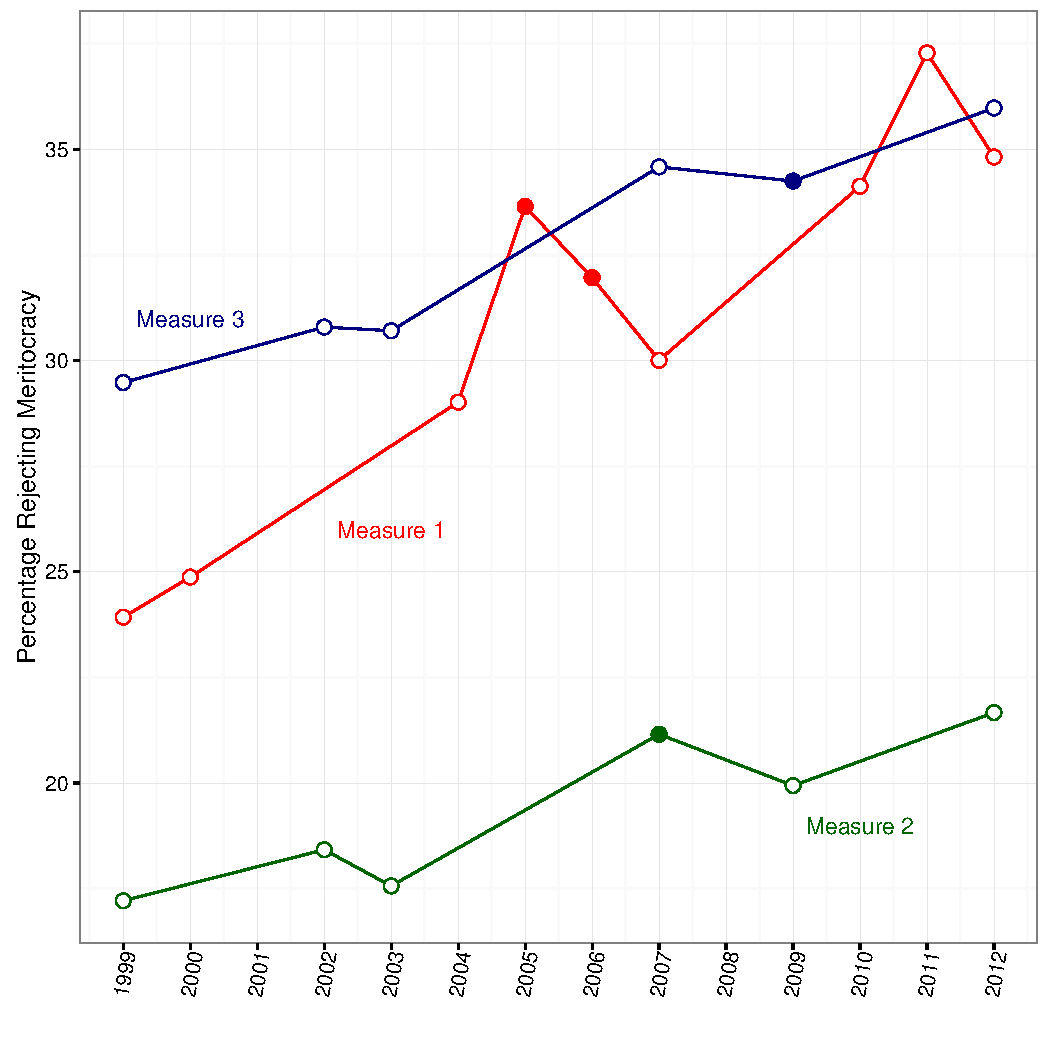
\includegraphics[width=5.25in]{../figures/04_three_measures_dv.pdf}
  \end{center}
  \begin{footnotesize}
  \begin{tabular}{p{.1in} p{5.1in}}
  & \emph{Notes}: The analyses presented in Table 1 of \citet[333]{Newman2015} were conducted on pooled observations with the dependent variable, rejection of meritocracy, measured in one of three different ways \citep[see][331]{Newman2015}.  Here, solid circles represent the data used by \citet{Newman2015}; hollow circles represent data in other available Pew surveys.  Plotting the percentage of (weighted) respondents to reject meritocracy by each of these measures reveals that the second measure results in much lower levels of rejection of meritocracy than either of the others and the third often yields considerably higher levels than the first.  In light of the evident lack of comparability of these three measures, pooling them into a single analysis cannot be justified.
  \end{tabular}
  \end{footnotesize}
\end{figure}

